\documentclass{isprs}

\usepackage{subfigure}
\usepackage{setspace}
\usepackage{graphicx}
\usepackage{geometry}
\usepackage{epstopdf}
\usepackage[labelsep=period]{caption}
\usepackage[british]{babel}
\usepackage[hang]{footmisc}
\usepackage{booktabs}
\usepackage{array}
\usepackage{siunitx}
\usepackage{url}
\def\footnotemargin{1em}

\geometry{a4paper, top=25mm, left=20mm, right=20mm, bottom=25mm, headsep=10mm, footskip=12mm}
\graphicspath{{figures/}}
\captionsetup{justification=centering,font=normal}
\captionsetup[figure]{font=small}
\captionsetup[table]{font=small}
\sisetup{
  round-mode=places,
  round-precision=3,
  detect-weight=true,
  detect-family=true
}

\title{From Coordinates to Geospatial Support: Uncertainty-Aware GIS for Vague Folklore Place Descriptions in a Japanese Yokai Archive}
\author{
Kosuke Shimizu\textsuperscript{1},
Hiroki Ichikura\textsuperscript{1},
Riri Ikebe\textsuperscript{2},
Mirai Hoshikawa\textsuperscript{1}
}
\address{
\textsuperscript{1 }University of Tsukuba, Japan\\
\textsuperscript{2 }Japan Women's University, Japan
}
\date{}

\begin{document}

\abstract{
The Kaii-Yokai Densho Database, maintained by the International Research Center for Japanese Studies (Nichibunken), records Japanese yokai folklore with a prefecture field and a short summary. The summary may contain formal place names, and it may also describe settings such as rivers, roads, houses, graves, and boundaries when no mappable toponym is given. A Folklore Geospatial Support Model is defined for this archive, representing each record by the evidence that supports spatial interpretation. The workflow transforms 33,378 records into resolution-aware geospatial features. All records receive prefecture-polygon support; 9,361 records (28.1\%) contain formal place mentions; 25,023 (75.0\%) contain place-description terms; and a conservative local GADM admin2 gazetteer upgrades 1,231 records (3.7\%). The admin2 subset reduces support area by a median 96.4\%. It also shows that coarser coordinates alter interpretation: 528 refined records (42.9\%) change coordinate-only terrain class relative to the prefecture-centroid baseline. Formal toponym extraction and place-description extraction are evaluated separately. A prefecture-stratified permutation model finds strong associations between category labels and rule-based place-function vocabulary within the archive, including Kappa (water spirits) with water-setting vocabulary, Yurei (ghosts) with death-ritual vocabulary, and Snake/Dragon (serpentine beings) with boundary-interface evidence. The result is a GIS representation for vague folklore places that keeps uncertainty, geospatial support, and human-environment boundary evidence available for inspection.
}

\keywords{Folklore geography, Geospatial support, Vague place descriptions, Digital humanities, Geographic uncertainty}

\maketitle
\sloppy

\section{Introduction}

Folklore scholarship has long connected yokai narratives to water, mountains, cultivation, shorelines, and settlement boundaries \cite{foster2015book}. Yanagita Kunio's account of cultural distribution also provides a precedent for treating regional variation as geographically meaningful \cite{yanagita1930kagyuko}.

The Kaii-Yokai Densho Database is maintained by the International Research Center for Japanese Studies (Nichibunken), a Japanese national research institute for Japanese studies. It contains Japanese yokai and uncanny folklore records with names, regional metadata, source references, and short summaries \cite{nichibun_yokai_database}. These fields support lookup by name or region. Spatial analysis needs another layer: the prefecture field, detected place names, place-description terms, polygon context, and confidence reason must remain distinguishable.

The Folklore Geospatial Support Model groups those inputs into evidence channels. A record can therefore carry a coordinate for display, a prefecture or municipality polygon as support area, and separate text-derived evidence about terrain, movement, dwelling, death ritual, or boundary settings.

Three questions guide the analysis. First, can vague folklore records be represented as multi-layer geospatial support? Second, how much does prefecture-centroid representation deform environmental interpretation when a subset can be refined to municipality support? Third, within prefectural strata, which yokai categories show above-background co-occurrence with rule-based place-function vocabulary such as water settings, routes, thresholds, livelihood, death-ritual, and taboo terms?

\section{Related Work and Motivation}

The problem belongs to geoparsing and spatial humanities, with an additional constraint from short folklore summaries. The record may contain a formal place name, a broad prefecture tag, or only a description of a setting.

Most geoparsing work begins with toponyms: systems identify place names, link them to gazetteers, and disambiguate candidate locations. HeidelPlace, for example, is framed around gazetteers, toponym recognition, and toponym resolution modules \cite{richter2017heidelplace}. Yokai summaries also contain non-toponymic place descriptions such as a bridge, pass, well, riverbank, village edge, grave, shrine, or house threshold. Work on vague places shows that uncertain place extent can be modelled \cite{jones2008vagueplaces}, while research on everyday place descriptions argues that place references and spatial relations should be represented together when gazetteers lack the relevant expressions \cite{chen2017everyday}. Historical geocoding similarly emphasizes that indirect spatial evidence carries textual, temporal, positional, and source uncertainty \cite{cura2018historical}.

Japanese administrative, river, lake, coastline, and elevation datasets provide the GIS context used for staged refinement \cite{gadm,naturalearth,mlit_ksj,mlit_admin,mlit_river,mlit_lake,mlit_elevation}. Location Reference Information and GeoNLP define a later path for local place evidence \cite{mlit_isj,geonlp}. These resources turn the prefecture-centroid baseline into a sequence of increasingly specific support areas.

\section{Data}

The input is a cleaned JSON export of the Kaii-Yokai Densho Database containing 33,378 records. The fields used here are the yokai or phenomenon name, major category, prefecture, source metadata, and short Japanese summary. The prefecture field gives every record an initial geographic anchor, while the summary supplies the text from which place mentions and terrain cues are extracted.

The category distribution is highly imbalanced. The residual Other class contains 19,084 records, while the largest named categories are Kitsune (fox figures; 3,618), Snake/Dragon (serpentine beings; 2,335), Yurei (ghosts; 1,641), Kappa (water spirits; 1,412), Tanuki (shapeshifting figures; 1,268), and Tengu (mountain beings; 1,224). This imbalance makes effect sizes and category-level diagnostics necessary, since statistical significance alone would mainly reflect sample size.

\section{System Pipeline}

\subsection{Prefecture-Centroid Georeferencing}

The first stage assigns a coordinate to every record using its structured \texttt{prefecture} field. The georeferencing module defines all 47 Japanese prefectures in a built-in centroid dictionary and appends latitude, longitude, and a geocoding-resolution field to each record. On the current cleaned dataset, all 33,378 records received prefecture-level coordinates.

This conservative baseline guarantees full coverage and defines the centroid as a metadata anchor for later, higher-resolution geocoding.

\subsection{Place Mention and Terrain Term Extraction}

The second stage applies GiNZA to the \texttt{summary} field \cite{ginza}. It stores formal place entities as \texttt{\_place\_mentions}. It also stores rule-based terrain words as \texttt{\_terrain\_terms}, grouped around mountain, water, coast, cultivation, route, and boundary vocabulary. The extraction script uses a JSON cache so that long runs can be resumed without repeating completed records.

The separation between formal place mentions and terrain terms is important for folklore text. Many summaries describe an environmental setting even when no municipality or landmark appears, so non-geocodable terrain words remain relevant to folklore-geographic questions about described settings.

\subsection{Folklore Geospatial Support Model}

The central representation is a geospatial-support object attached to every record. It stores the prefecture or municipality polygon that supports a record, detected formal place names, place-description terms, terrain evidence, human-condition terms, source metadata, resolution level, and confidence reason. Toponym support stores detected place names and whether they resolve to a unique local municipality candidate. Terrain support stores coordinate-only and text-aware labels separately.

Place-description support records functional spatial vocabulary in seven groups: water setting, mobility, boundary, livelihood, dwelling, death-ritual, and taboo/time/weather. A separate human-condition channel records actors and actions. The model derives strict boundary-interface types when environmental terms co-occur with human-use terms: water crossing, waterside boundary, water danger norm, mountain route, mountain boundary, coastal landing, domestic threshold, mortuary boundary, and water livelihood. A broader human-environment interface flag is retained as a looser diagnostic. These fields separate natural-feature vocabulary from record-level combinations of environmental and human-use vocabulary.

\begin{center}
\centering
\captionof{table}{Fields in the Folklore Geospatial Support Model.}
\label{tab:support-model}
\footnotesize
\setlength{\tabcolsep}{3pt}
\begin{tabular}{p{0.27\linewidth}p{0.56\linewidth}}
\toprule
Support channel & Evidence stored \\
\midrule
Administrative & Prefecture or admin2 polygon, support area, resolution level. \\
Toponym & Detected formal place names, resolved candidate, matching method. \\
Place-description & Water setting, mobility, boundary, livelihood, dwelling, death, taboo terms. \\
Terrain & Coordinate-only and text-aware terrain labels, source GIS layers. \\
Human condition & Actors and actions mentioned in the summary. \\
Interface & Derived boundary/contact types such as water crossing or domestic threshold. \\
Confidence & Reason for support: exact match, unresolved toponym, text cue, metadata only. \\
\bottomrule
\end{tabular}
\end{center}

\subsection{Local Admin2 Gazetteer Refinement}

The pipeline attempts a local municipality-level refinement against GADM level 2 names. The implementation filters GADM records to municipality-like units, including cities, towns, villages, special wards, and related local administrative types. It then searches each summary for official Japanese municipality names within the record's prefecture and separately matches extracted place mentions against the same prefecture-bounded gazetteer. A record is upgraded only when exactly one municipality candidate is found; ambiguous records remain at prefecture resolution.

This refinement upgraded 1,231 records, or 3.7\% of the archive, to local GADM admin2 representative points. Of these, 329 were matched directly from summary text and 902 from extracted place mentions. The remaining 32,147 records keep their prefecture-centroid coordinates. The reported experiment is therefore a mixed-resolution representation that records whether each point is prefecture-level or municipality-level through \texttt{\_geo\_level}.

\subsection{Terrain and Polygon GIS Enrichment}

The enrichment module downloads and caches GADM v4.1 Japan level 2 administrative boundaries, Natural Earth coastline and lake layers, and National Land Numerical Information River Data (W05), a Japanese river centre-line dataset \cite{gadm,naturalearth,mlit_river}. The W05 loader resolves prefecture-specific source files, extracts the \texttt{Stream.shp} layers, converts JGD2000 geometries to EPSG:4326, and merges 286,436 river features into a local cache. It then joins each point to a GADM level 2 unit and computes nearest distances to W05 rivers, Natural Earth lakes, and coastlines in a projected coordinate reference system.

Because most reported points in this experiment remain prefecture centroids, the module also computes GIS features at the matching prefecture-polygon support. GADM level 2 polygons are dissolved to prefectures, and each prefecture receives area, coastline length per 1,000 km\textsuperscript{2}, W05 river length per 1,000 km\textsuperscript{2}, and lake-area share. These polygon metrics are coarse. They describe prefecture-level geographic context for records still at prefecture level, while the subset of locally refined records carries municipality-level coordinates.

For the locally refined subset, the same polygon-context calculation is repeated at GADM admin2 support. The implementation first identifies the admin2 units actually used by municipality-level records, then clips W05 rivers, Natural Earth coastline, and Natural Earth lakes to those target polygons. This targeted calculation adds admin2 area, river density, coastline density, and lake-area share to the 1,231 refined records.

The classifier writes two terrain representations. The coordinate-only representation uses only the point location and GIS layers: records within 10 km of the Natural Earth coastline are labelled coastal; inland records more than 50 km from the coast and within 2 km of W05 rivers are labelled valley; records within 0.5 km of water are labelled inland-water; and the remaining records are labelled plain. The valley label is a river-proximal inland proxy, since elevation and slope are not used in the reported run. The text-aware representation begins from the same coordinate-only label and then allows extracted terrain terms to add mountain, inland-water, or coastal narrative cues. The original \texttt{\_terrain\_class} field is retained as the text-aware label for backwards compatibility, while \texttt{\_terrain\_coord\_only} and \texttt{\_terrain\_text\_aware} keep the two evidential bases separate.

The rules are coarse and traceable: every label comes from either a GIS threshold or an extracted terrain cue. That separation prepares the representation for later elevation, slope, land-use, historical-boundary, or higher-resolution gazetteer layers.

\section{Experiments}

\subsection{Reproducible Setup}

The experiment module reads the enriched archive and writes the statistical summaries and figures. The current run used prefecture centroids for 32,147 records and local GADM admin2 representative points for 1,231 records, with W05 river centre-lines as the river layer. Its main diagnostic compares coordinate-only and text-aware terrain representations. The split keeps GIS thresholds and summary-term evidence in separate fields.

\subsection{Geospatial-Support Coverage}

Coverage is reported for each evidence channel. Formal toponym extraction covers 9,361 records (28.1\%), while place-description terms cover 25,023 records (75.0\%). Terrain terms cover 20,242 records (60.6\%), human-condition terms cover 16,066 (48.1\%), strict boundary-interface terms cover 9,047 (27.1\%), and a broader human-environment interface flag covers 16,102 records (48.2\%).

Figure~\ref{fig:support-stage} summarizes this coverage. The local admin2 gazetteer covers only 1,231 records, but it reduces their median support area to 213.6 km\textsuperscript{2}, a 96.4\% median reduction from prefecture scale. Even sparse municipality refinement therefore provides a diagnostic subset for measuring how much coarse metadata changes coordinate-derived interpretation.

\begin{figure}[tbp]
\centering
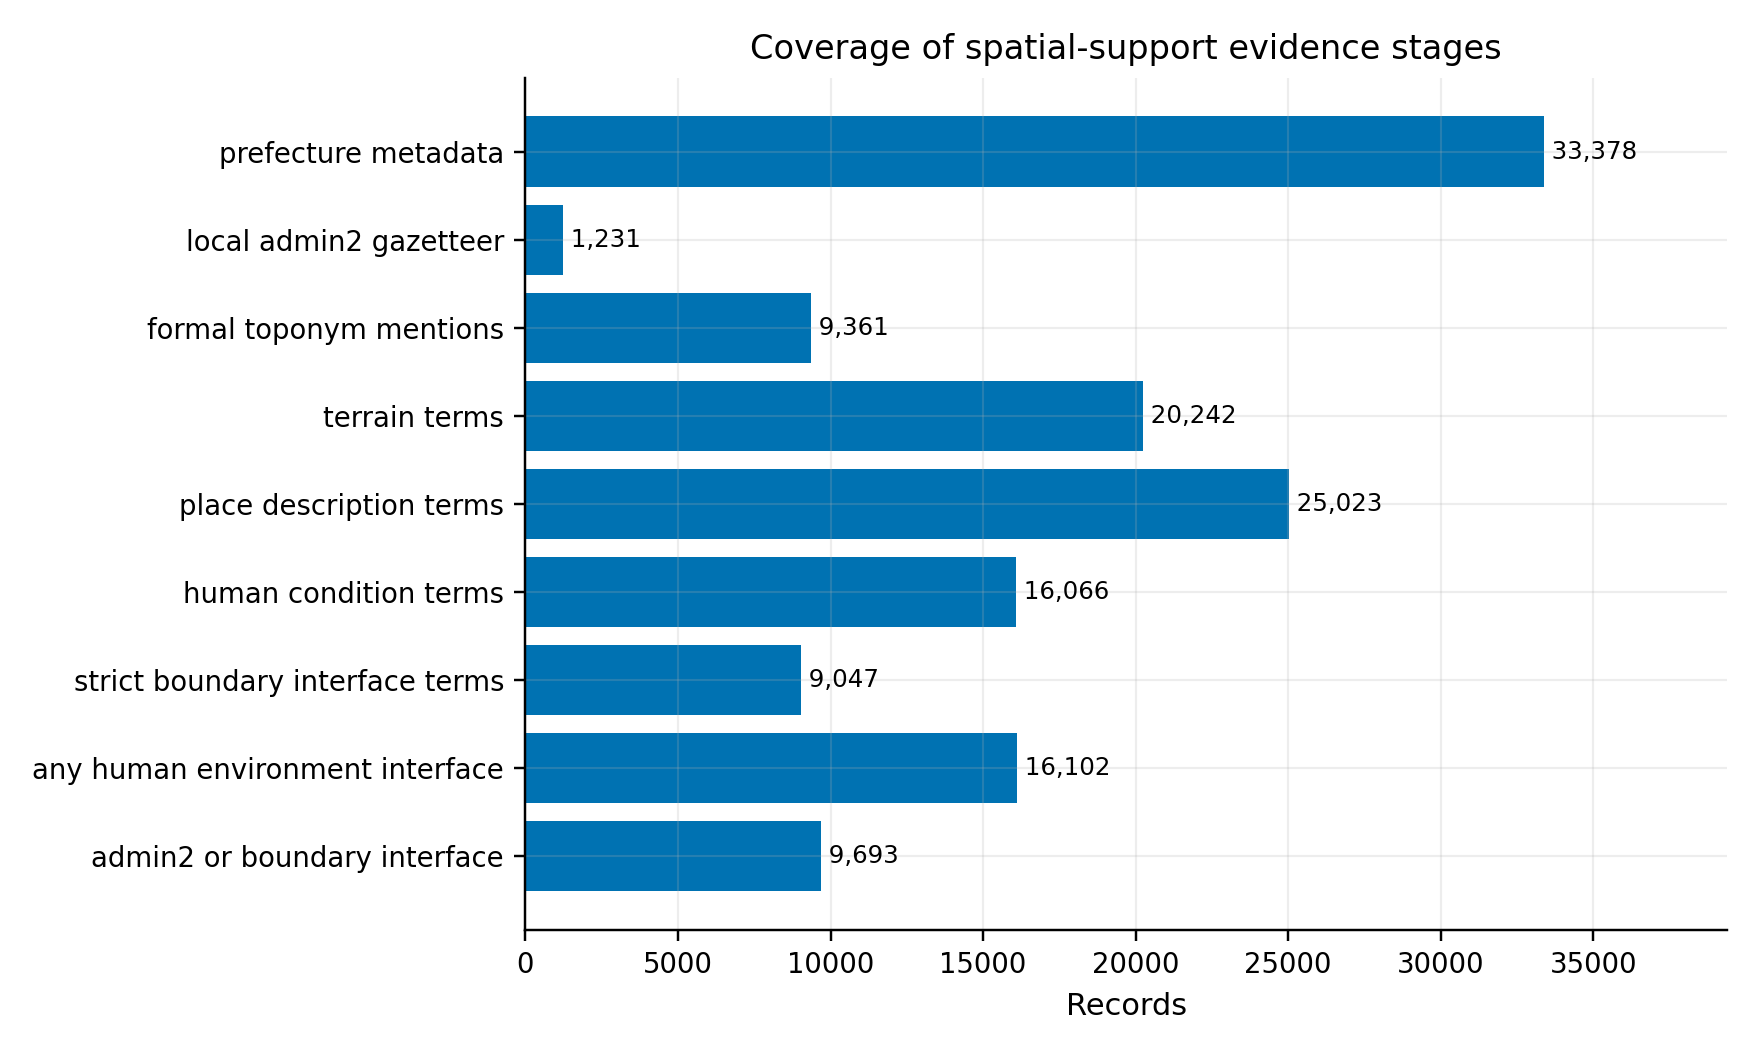
\includegraphics[width=\linewidth]{fig_spatial_support_stage_coverage.png}
\caption{Coverage of geospatial-support evidence channels. Place-description evidence covers more records than formal toponyms.}
\label{fig:support-stage}
\end{figure}

\subsection{Coordinate-Only and Text-Aware Terrain Labels}

The enrichment stage produced the two terrain representations shown in Table~\ref{tab:terrain-counts}. The coordinate-only baseline is dominated by the geometry of prefecture centroids, with 1,231 records using locally refined municipality coordinates: 17,747 records are labelled coastal, 7,199 valley, 4,824 plain, and 3,608 inland-water. Most coordinate-only results describe metadata coordinates.

The text-aware representation changes 11,516 labels, or 34.5\% of the archive. The largest off-diagonal transitions are coastal to mountain (4,635 records), valley to mountain (1,990 records), and plain to mountain (1,451 records). The transitions measure terrain cues in summaries that the coordinate representation cannot express.

A direct centroid-bias diagnostic confirms the baseline mechanism. Among the 47 prefecture centroids, 28 are classified as coastal, 8 as plain, 7 as valley, and 4 as inland-water. Since 96.3\% of records still inherit prefecture-level coordinates in the reported run, most records in a prefecture share the same coordinate-derived terrain context regardless of within-prefecture topographic diversity. The \texttt{\_geo\_level} field exists to keep this resolution visible in both the interface and the analysis.

\begin{figure}[tbp]
\centering
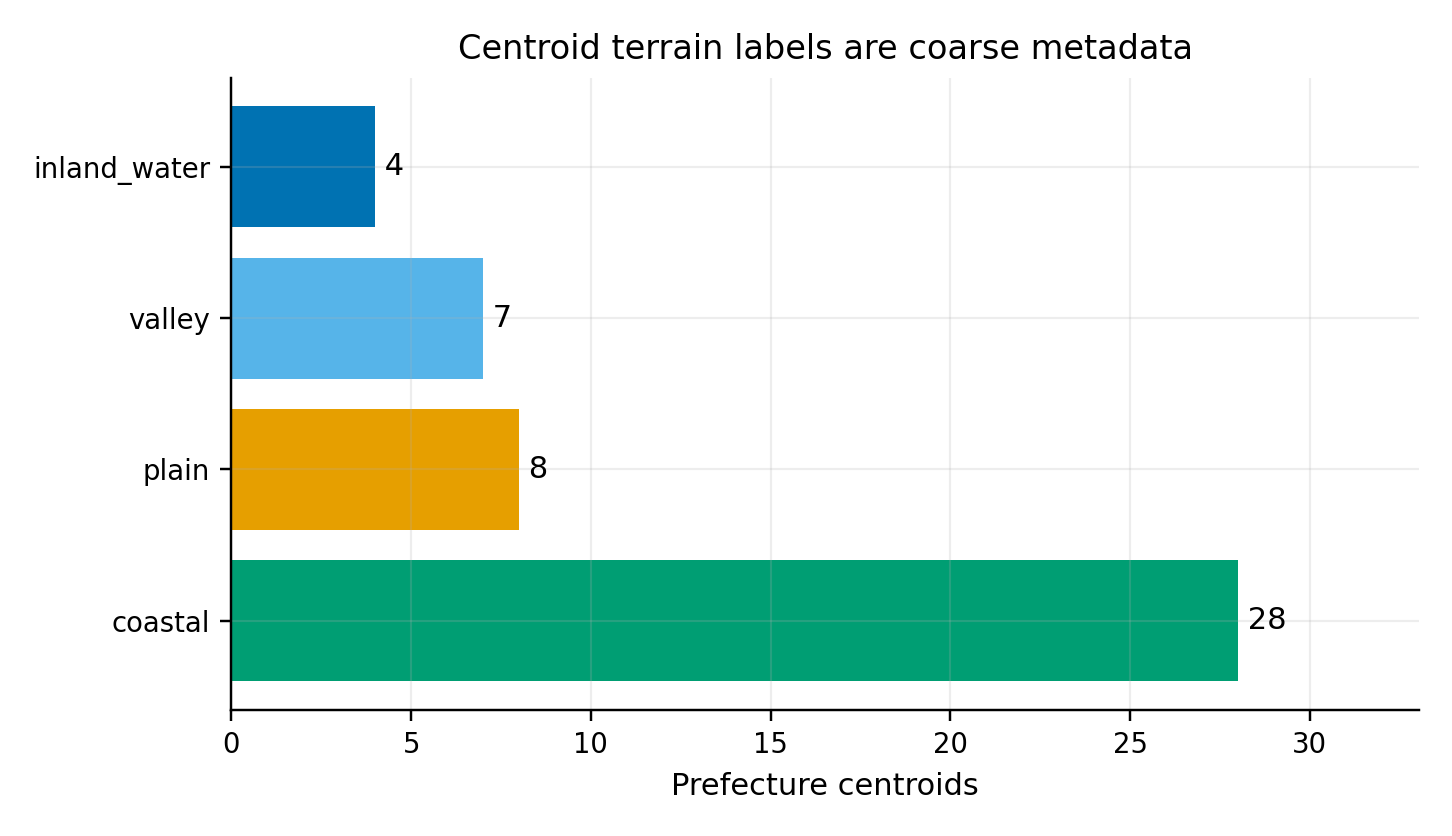
\includegraphics[width=0.62\linewidth]{fig_prefecture_centroid_bias.png}
\caption{Coordinate-only labels assigned to the 47 prefecture centroids. This diagnostic shows the dominant metadata geography still present after local admin2 refinement.}
\label{fig:centroid-bias}
\end{figure}

\begin{table}[tbp]
\centering
\caption{Coordinate-only and text-aware terrain labels in the mixed-resolution experiment.}
\label{tab:terrain-counts}
\footnotesize
\setlength{\tabcolsep}{3pt}
\begin{tabular}{lrrrr}
\toprule
Label & Coord. n & Coord. \% & Text n & Text \% \\
\midrule
Coastal & 17,747 & 53.17\% & 13,460 & 40.33\% \\
Plain & 4,824 & 14.45\% & 2,337 & 7.00\% \\
Valley & 7,199 & 21.57\% & 3,987 & 11.94\% \\
Mountain & 0 & 0.00\% & 9,156 & 27.43\% \\
Inland-water & 3,608 & 10.81\% & 4,438 & 13.30\% \\
\bottomrule
\end{tabular}
\end{table}

\begin{figure}[tbp]
\centering
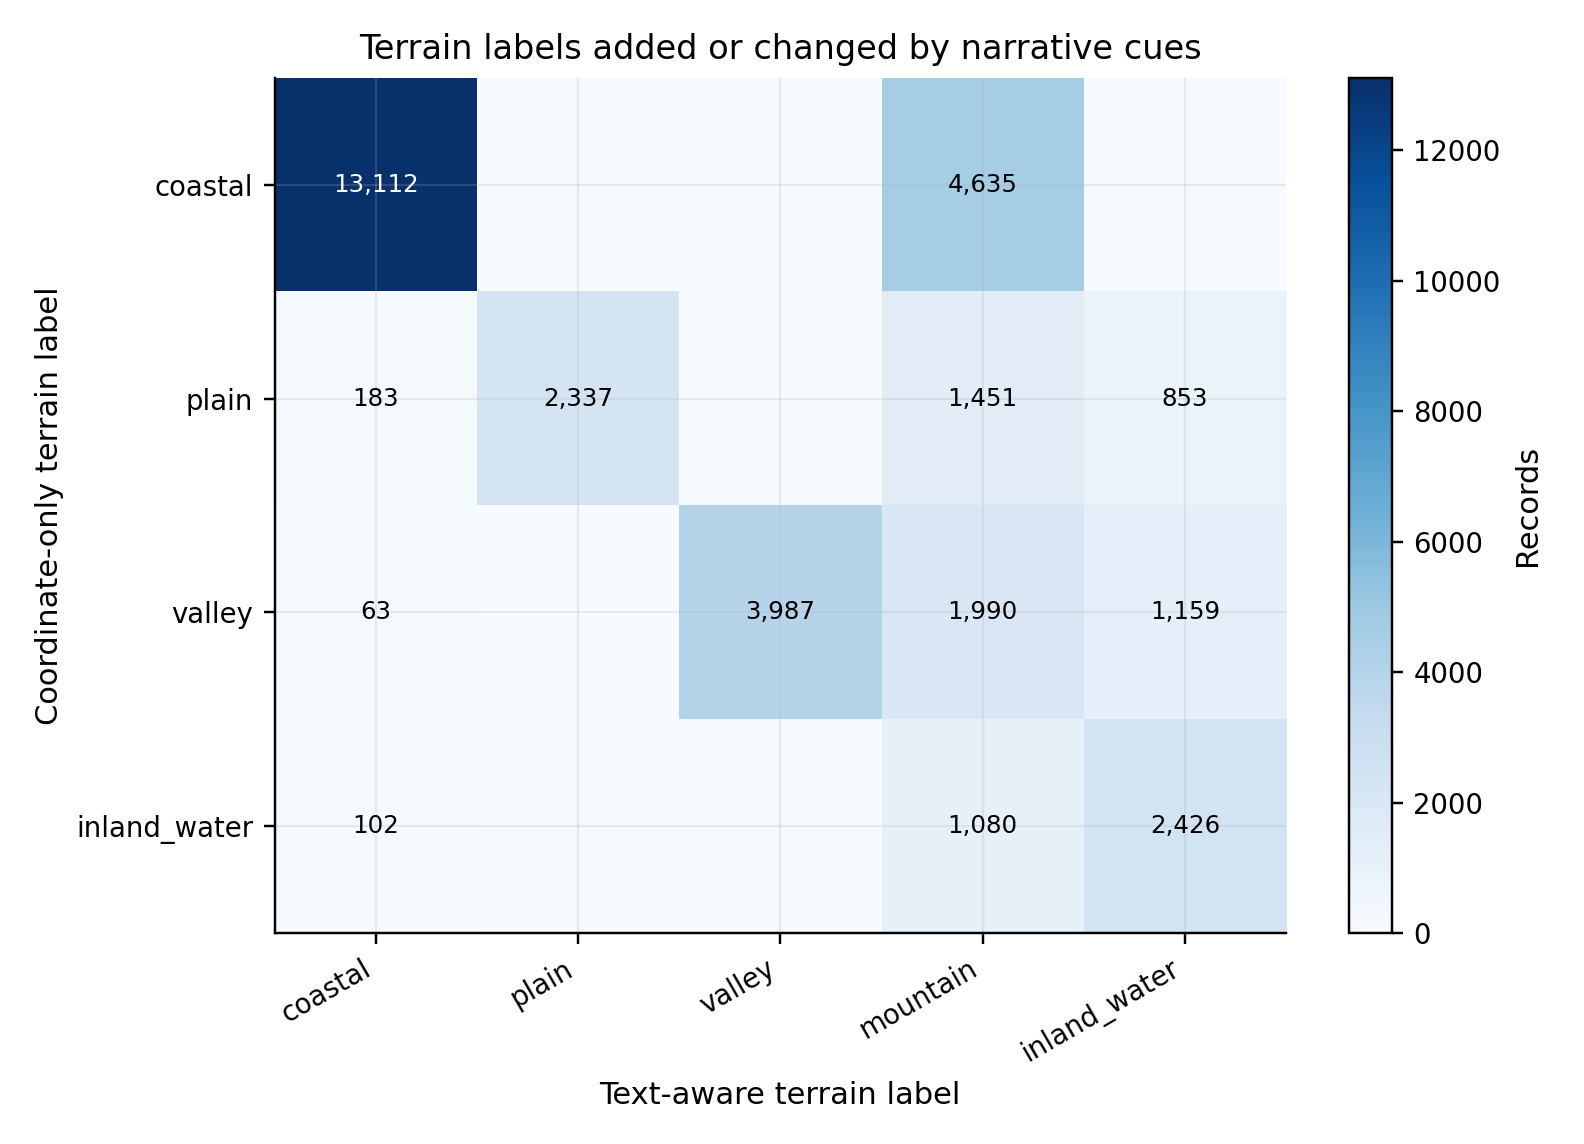
\includegraphics[width=0.82\linewidth]{fig_terrain_representation_transition.png}
\caption{Transition matrix from coordinate-only labels to text-aware labels. The largest off-diagonal cells show where summary-derived terrain cues add information that prefecture centroids cannot represent.}
\label{fig:terrain-transition}
\end{figure}

\subsection{Prefecture-Polygon GIS Context}

The centroid labels above are diagnostic. Figure~\ref{fig:pref-gis-context} plots the 47 prefectures by coastline density and W05 river density, with point size proportional to record count and colour showing lake-area share. A record assigned only to a prefecture inherits that prefecture's polygon context; locally matched records additionally carry municipality coordinates.

Across prefectures, W05 river density ranges from 545.9 to 1,367.3 km per 1,000 km\textsuperscript{2}, coastline density ranges from 0 to 152.6 km per 1,000 km\textsuperscript{2}, and the largest lake-area share is Shiga at 16.48\%. These metrics describe the polygon support inherited by records that remain at prefecture level.

\begin{figure}[tbp]
\centering
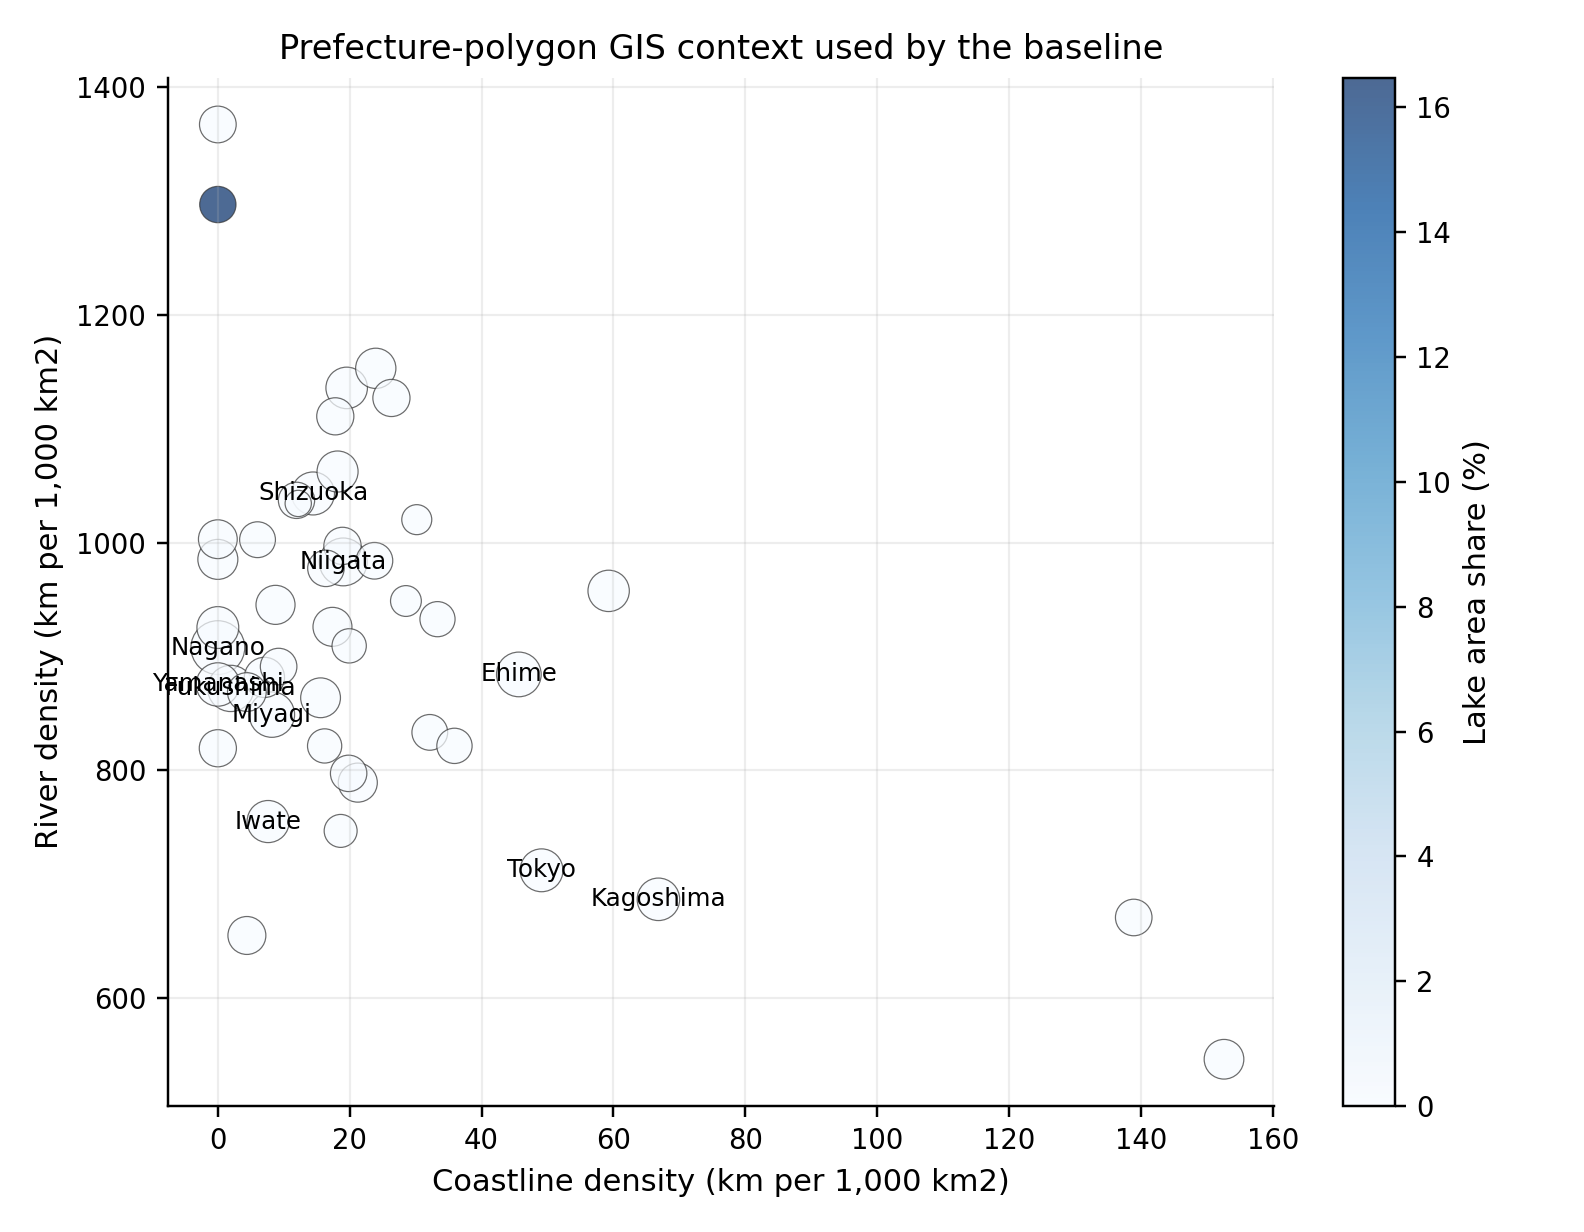
\includegraphics[width=0.82\linewidth]{fig_prefecture_gis_context.png}
\caption{Prefecture-polygon GIS context used in the baseline. The features are computed from GADM prefecture polygons, Natural Earth coast/lake data, and National Land Numerical Information River Data (W05).}
\label{fig:pref-gis-context}
\end{figure}

\subsection{Admin2 Refinement as a Distortion Test}

The 1,231 locally refined records serve as a diagnostic set for RQ2. For each refined record, we compare the coordinate-only terrain class inherited from its prefecture centroid with the coordinate-only class computed at its admin2 representative point. In 528 refined records (42.9\%), the terrain class changes. The most common changes are coastal to inland-water (205 records), coastal to plain (89), plain to inland-water (65), valley to inland-water (52), and plain to coastal (45). Median support-area reduction is 96.4\%. Median coast distance increases by 3.7 km in the refined subset, and median water distance decreases by 0.09 km. The subset is produced by successful local name matching, so the result is a distortion diagnostic for the refined records rather than an archive-wide accuracy estimate.

\begin{figure}[tbp]
\centering
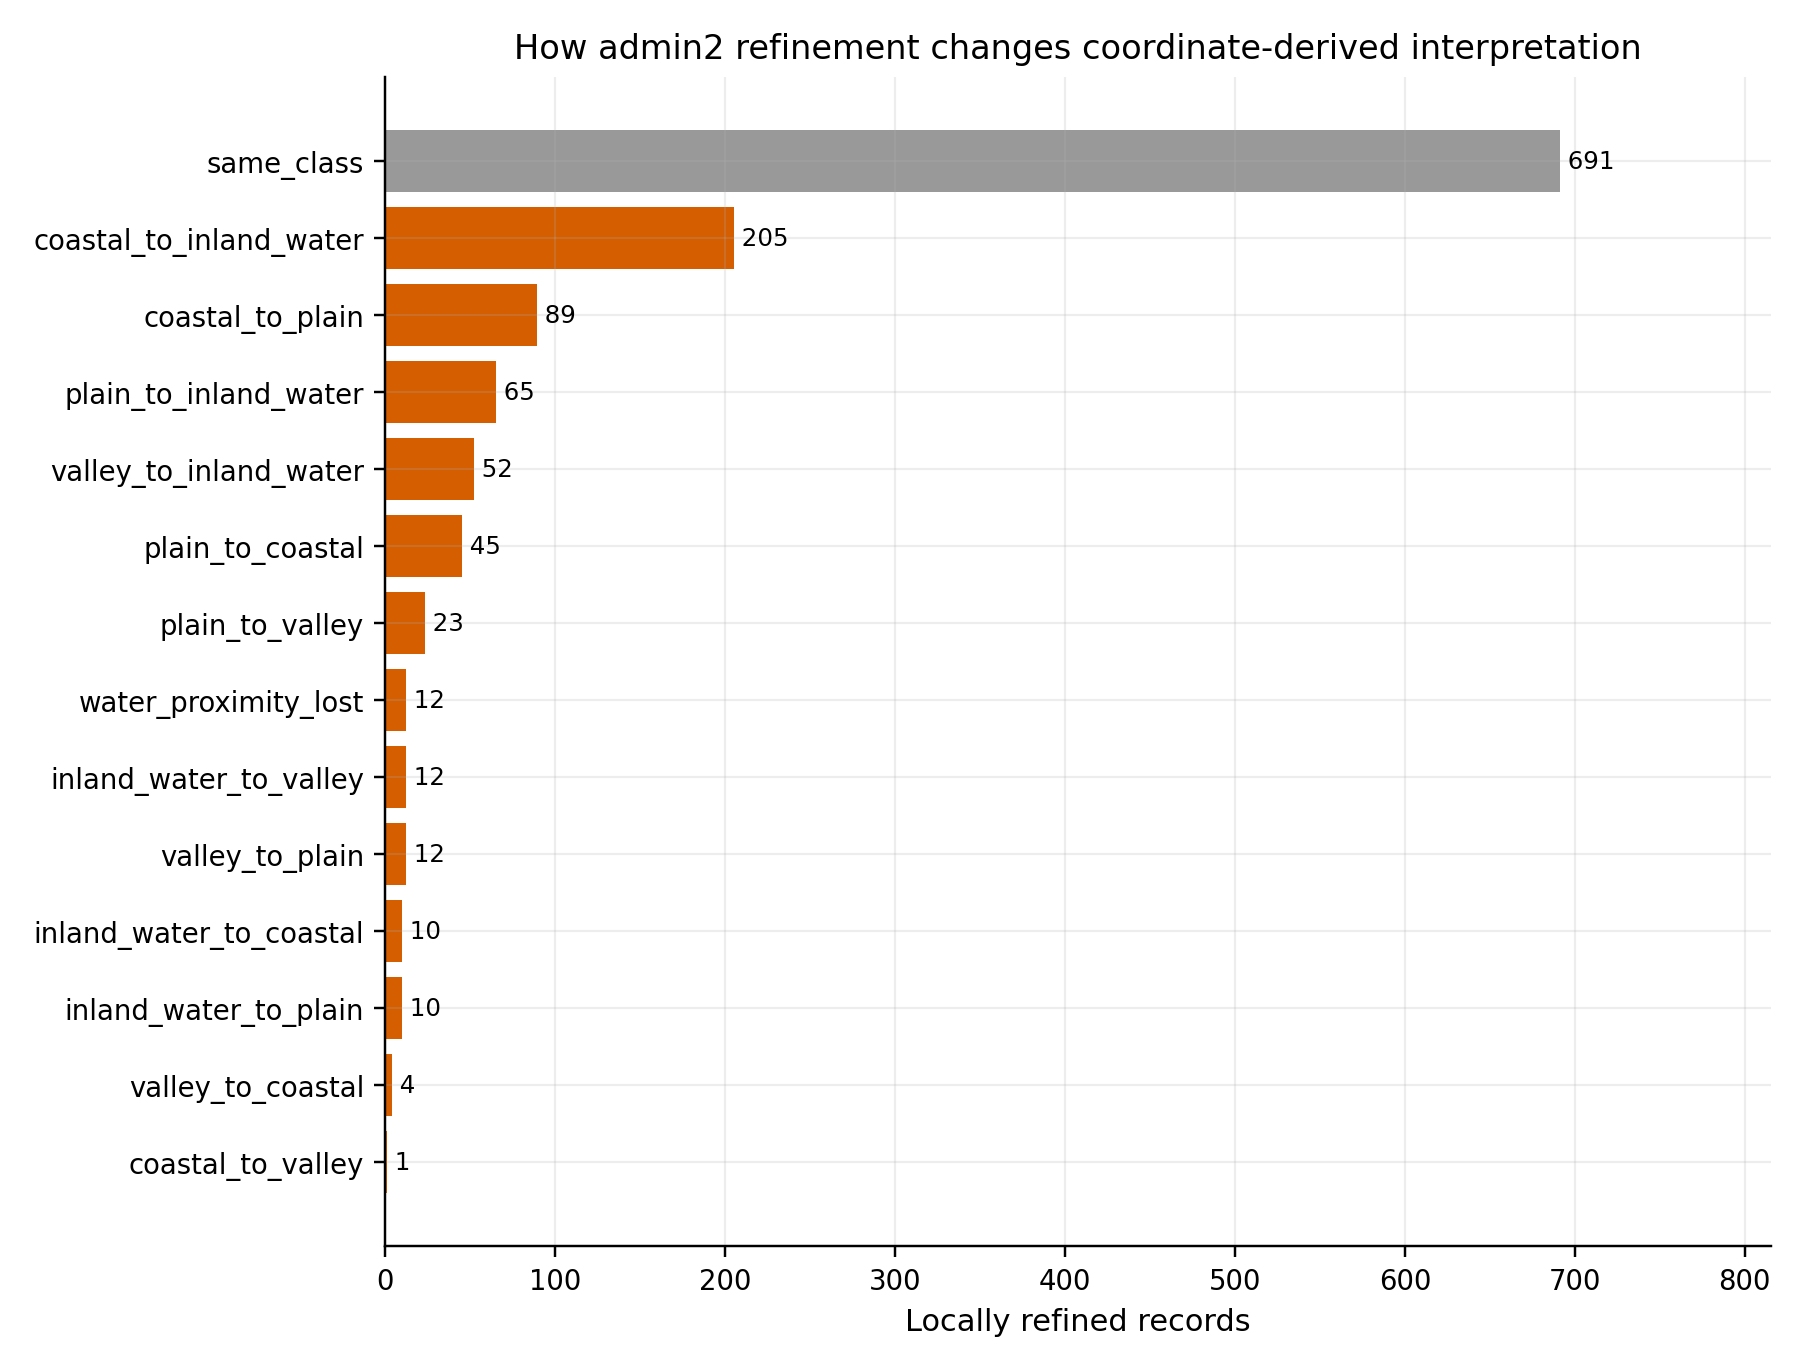
\includegraphics[width=0.82\linewidth]{fig_admin2_refinement_distortion.png}
\caption{Changes in coordinate-derived interpretation when the 1,231 locally refined records move from prefecture-centroid support to admin2 support.}
\label{fig:admin2-distortion}
\end{figure}

\subsection{Place-Function Associations Under a Null Model}

RQ3 is tested on place-function term incidence. The analysis uses a prefecture-stratified permutation null model: category labels are shuffled within each prefecture, preserving prefecture composition while breaking category-specific association with place-function terms. The test asks whether Kappa records, for example, contain water-setting terms more often than expected among records from the same prefectures. The unit of analysis is record-level term incidence in summaries. Physical proximity is evaluated separately on the admin2 subset below.

Figure~\ref{fig:null-model} shows the resulting z-scores over 500 permutations. The strongest positive associations are Yurei with death-ritual vocabulary (observed 1,233, expected 264.9, observed/expected ratio 4.65), Kappa with water-setting vocabulary (1,101 vs. 326.5, ratio 3.37), Snake/Dragon with water-setting vocabulary (1,090 vs. 488.3, ratio 2.23), and Snake/Dragon with strict boundary-interface terms (930 vs. 632.6, ratio 1.47). Kappa is also positively associated with strict boundary-interface terms (591 vs. 385.3, ratio 1.53) and livelihood terms (398 vs. 270.6, ratio 1.47). The z-scores rank cells; the observed/expected ratios give the more interpretable effect summaries. Within the same prefectures, Kappa and Snake/Dragon summaries disproportionately contain water-setting and interface vocabulary, and Yurei summaries disproportionately contain death-ritual vocabulary.

An admin2-only water-feature diagnostic tests the same category on the 1,231 locally refined records. The distance field uses the same nearest-water layer as the enrichment pipeline: MLIT W05 rivers plus Natural Earth lakes. Among the 48 locally refined Kappa records, the observed median distance to the nearest water feature is 0.371 km. A prefecture-stratified category-shuffle null with 10,000 permutations expects a median of 0.295 km ($p=0.936$ for a smaller median). The observed median is larger than the shuffle expectation, so the Kappa result is treated as summary evidence.

\begin{figure}[tbp]
\centering
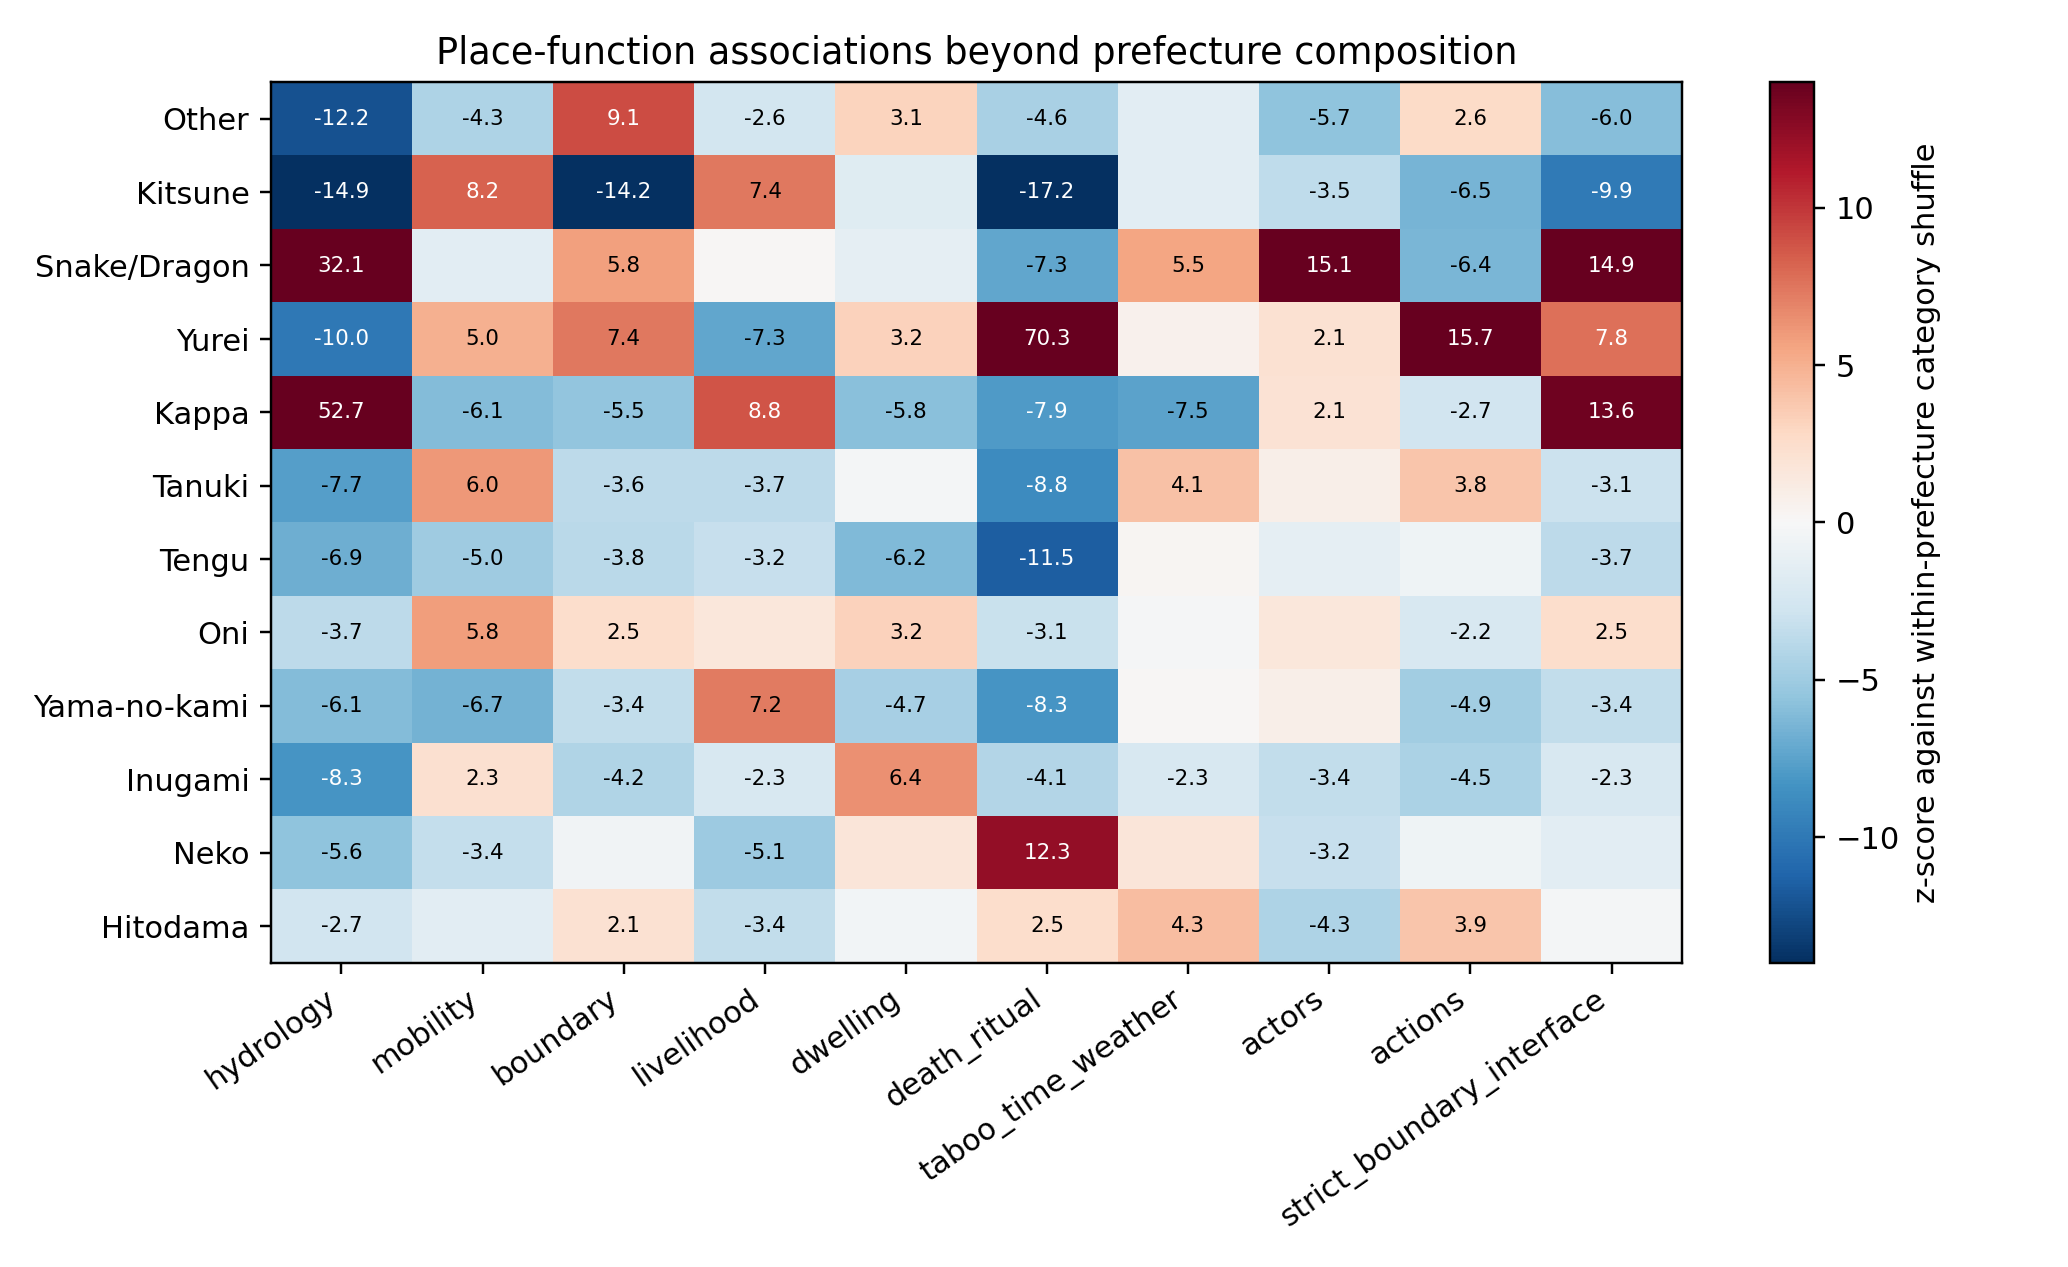
\includegraphics[width=\linewidth]{fig_place_function_null_residuals.png}
\caption{Place-function associations after shuffling category labels within prefectures. Positive cells show category-function links that exceed prefectural background composition.}
\label{fig:null-model}
\end{figure}

\subsection{Robustness Diagnostics}

The robustness diagnostics target leakage and sensitivity in the geospatial-support representation. All dictionaries, intermediate evidence fields, and rule outputs are inspectable. The checks below rerun the strongest associations under category-name masking, dictionary sensitivity, interface-definition ablation, and prefecture-stratified permutation tests.

\begin{table}[tbp]
\centering
\caption{Extraction and support diagnostics on 33,378 records. The table reports evidence-channel coverage.}
\label{tab:extraction-diagnostics}
\footnotesize
\setlength{\tabcolsep}{3pt}
\begin{tabular}{p{0.50\linewidth}p{0.34\linewidth}}
\toprule
Diagnostic & Value \\
\midrule
Records in extraction run & 33,378 \\
Records with place mentions & 9,361 (28.1\%) \\
Records with terrain terms & 20,242 (60.6\%) \\
Records with place-description terms & 25,023 (75.0\%) \\
Records with strict boundary-interface terms & 9,047 (27.1\%) \\
Records with any human-environment interface & 16,102 (48.2\%) \\
Unique prefecture-place candidate keys & 9,015 \\
Local admin2-refined records & 1,231 (3.7\%) \\
Admin2 records with changed coord.-terrain interpretation & 528 (42.9\% of refined records) \\
Coordinate-only terrain labels & coastal 17,747; valley 7,199; plain 4,824; inland-water 3,608 \\
Text-aware terrain labels & coastal 13,460; mountain 9,156; inland-water 4,438; valley 3,987; plain 2,337 \\
Labels changed by terrain terms & 11,516 (34.5\%) \\
\bottomrule
\end{tabular}
\end{table}

Table~\ref{tab:robustness} reports the three most important robustness checks. First, category-specific surface forms such as kappa, tengu, kitsune, yurei, and snake/dragon terms are masked from summaries before place-function extraction; this affected 13,140 summaries and removed 22,974 surface-form occurrences. Second, 10\%, 20\%, and 30\% of terms are randomly removed from each dictionary group, with five seeded lexical drops per rate. Third, the boundary-interface feature is recomputed under broad, strict, and conservative definitions: broad uses any environmental term plus human-condition term, strict uses the co-occurrence-derived interface types defined above, and conservative removes the water-danger-norm interface from the strict set.

Across these diagnostics, the focal associations remain positive, with changing magnitudes. Category-name masking reduces the Kappa/water-setting and Yurei/death-ritual z-scores, yet both remain large. Dictionary deletion affects the death-ritual association most strongly at 30\% removal, and Snake/Dragon boundary-interface evidence remains positive under all interface definitions. The focal results survive category-name masking, dictionary deletion, and interface-definition changes.

\begin{table}[tbp]
\centering
\caption{Robustness diagnostics for key z-scores under prefecture-stratified null models: Kappa-water-setting, Yurei-death-ritual, and Snake/Dragon-boundary-interface. Dictionary-drop rows report median z-scores over five seeded lexical drops; interquartile ranges are released in the accompanying CSV output.}
\label{tab:robustness}
\scriptsize
\setlength{\tabcolsep}{2pt}
\begin{tabular}{lrrr}
\toprule
Condition & Kappa water & Yurei death & Snake bound. \\
\midrule
Full & 52.7 & 70.3 & 14.9 \\
Name masked & 33.7 & 45.1 & 15.4 \\
Drop 10\% & 54.4 & 70.7 & 12.7 \\
Drop 20\% & 54.4 & 72.2 & 11.7 \\
Drop 30\% & 58.6 & 26.0 & 12.9 \\
Broad & 52.7 & 70.3 & 18.7 \\
Strict & 52.7 & 70.3 & 14.9 \\
Conservative & 52.7 & 70.3 & 9.8 \\
\bottomrule
\end{tabular}
\end{table}

\section{Discussion}

The results make the resolution of each spatial statement visible. Prefecture metadata supports complete national coverage, admin2 matching supplies a small diagnostic subset, and text-derived place-function terms supply evidence about how summaries describe settings. Keeping these channels separate prevents centroid terrain labels, summary vocabulary, and polygon context from being read as the same kind of evidence.

The category-place-function analysis describes archive language. Kappa records are associated with water-setting, strict boundary-interface, and livelihood terms. Snake/Dragon records combine water-setting, actors, and boundary-interface evidence. Yurei records are dominated by death-ritual vocabulary. The admin2 water-distance diagnostic bounds that interpretation: the Kappa subset has a larger observed median water-feature distance than the within-prefecture shuffle expectation. Human-environment interface language is therefore a useful evidence channel, and physical placement requires finer geocoding.

The admin2 distortion test gives the spatial result a narrower and more defensible form. Coarse metadata does more than increase uncertainty: in the locally refined subset, it changes coordinate-derived terrain labels for 42.9\% of records. The refined subset is selected by successful local name matching, so the percentage describes this subset. Its value is diagnostic: it shows where prefecture-centroid maps can change the environmental reading of records that contain enough information for municipality-level support.

\section{Limitations}

The reported experiment uses prefecture support for 96.3\% of records. Coordinate-only terrain labels mainly describe prefecture-level metadata, with a small municipality-level supplement from local GADM matching. Place-description and boundary-interface labels are rule-based summary evidence. The paper therefore reports support area, coordinate evidence, text evidence, and confidence reason separately.

The water-feature layer uses W05 river centre-lines, Natural Earth lakes, and Natural Earth coastlines. Irrigation canals, village streams, ponds, springs, wells, and small sacred water sites remain underrepresented. Summaries also contain ambiguous local names, obsolete place names, shrine names, and terrain descriptions without formal toponyms. These gaps affect both spatial refinement and rule-based extraction.

The source archive is a constructed collection. Record density reflects collection history, publication practices, source survival, and database construction. Spatial density is therefore archive density unless normalized against source availability and collection process.

\section{Conclusion}

The Folklore Geospatial Support Model converts 33,378 records from the Kaii-Yokai Densho Database into evidence channels for prefecture or municipality support, formal place mentions, place-description terms, terrain evidence, human-condition terms, boundary-interface types, and confidence reason. Formal toponyms occur in 28.1\% of records, while place-description terms occur in 75.0\%. Local admin2 refinement covers 1,231 records, reduces support area by a median 96.4\%, and changes coordinate-derived terrain interpretation for 42.9\% of refined records.

The archive-level analysis is strongest when the evidence channels remain separate. Category-to-place-function associations persist beyond prefectural composition, including Kappa/water-setting, Yurei/death-ritual, and Snake/Dragon/boundary-interface evidence. The admin2 water-distance diagnostic separates the Kappa text association from physical water proximity. The resulting GIS representation keeps vague folklore places analyzable while avoiding a single asserted event point for every record.

\bibliography{refs}

\end{document}
